%Bioinformatics presentation
\documentclass{beamer}
\usepackage{graphicx,tabto}
\usepackage{amsmath,amsfonts,amssymb}
%exclude navigation symbols
\beamertemplatenavigationsymbolsempty
\usetheme[compress]{Dresden}
\usecolortheme{seagull}
\usefonttheme{structurebold}
\expandafter\def\expandafter\insertshorttitle\expandafter{\hfill\insertframenumber\,/\,\inserttotalframenumber}
\title{Comparing forward/reverse strand exonic and intronic RNA secondary structures, for PHO1-2 Oryza sativa transcript orthologs}
\author{Mario and Ramona}
\institute[TBI]{Institute for Theoretical Chemistry\\ University of Vienna}
\date{\today}


\begin{document}
\frame{
  \titlepage
}


\frame{
\frametitle{Introduction}
	water stress in O.sativa:	
	\begin{itemize}
	\item  normal levels of PHO1-2 mRNA
	\item  high levels of antisense mRNA, and PHO1-2 protein\\~\\
	
	\end{itemize}
	
	Question: translation regulation via secondary structures, binding of antisense to the mRNA transcript?  
	
}

%If put under water stress, O.sativa expresses normal levels of PHO1-2 mRNA, but high level of its antisense RNA, but leading to higher PHO1-2 protein levels.
%Maybe antisense RNA regulates gen expression by formation of secondary structures, on translation level, by binding to the PHO1-2 mRNA transcript.
%This kind of regulation takes place on a RNA level, meaning that the RNA secondary structure might play a very important role. This is why we tried to find 
%evolutionary conserved functional RNA secondary structures via bioinformatic algorithms. Furthermore we were curious to find the difference between RNA secondary structures formed by either exonic or intronic regions. 


\frame{
  \frametitle{Workflow}
\begin{center}
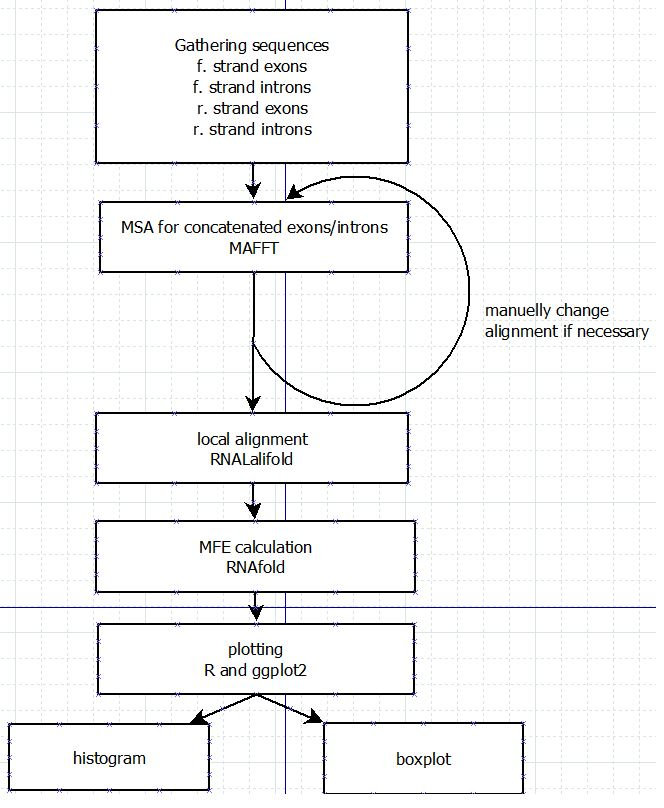
\includegraphics[width=0.5\textwidth]{./pictures/workFlow.png}
\end{center}
}

%Flow chart slide
%
%Prior to starting our calculations and analysis, we created a flowchart of our future tasks, as shown on this slide.
%Of course we started with the gathering of the input sequences. Data was taken from the ensemble database, in detail the PHO1-2 gene transcript from Oryza sativa and their corresponding ortholog transcript. Overall, 10 orthologs of the Oryza family were used for this analysis. For analysis, the forward strands were taken and converted to the reverse complementary strands via pearl scripts. We restricted the whole genomic sequence, by taking only the EXONs and concatenated these sequences to one big EXON file for every ortholog. Subsequently we performed the same steps for the Introns. 
%The next step was obtaining a multiple sequence alignment for our sequences, by using the program MAFFT. MAFFT was executed with the --auto parameter. We inspected the alignments manually with different MSA viewers and if necessary we were willing to optimize the alignments. For this analysis, no optimization was performed by us.
%Afterwards, locally stable RNA structures should be found for our given multiple sequence alignment and therefore the RNALalifold algorithm fits perfectly for this task. RNALalifold was executed with a span parameter of 100 and resulted with all found locally secondary structures, plus their corresponding free energy. At last, the outcome of all MFE values found in the concatenated EXONS and INTRONS of each ortholog was plotted with the R extension tool ggplot2. For our presentation, histograms and boxplots are fitting diagrams for showing our result.


\frame{
\frametitle{MAFFT}

\begin{itemize}
\item multiple sequence alignment with fast fourier transform
\item works with vectores: 
 \tabto{2cm} AA:
 \tabto{4cm} v(a) volume and p(a) polarity
 \tabto{2cm} nucleotide:
 \tabto{4cm} frequency of bases at each column
\item peaks for homologous regions

\end{itemize}
}

\frame{
  \frametitle{MAFFT}
  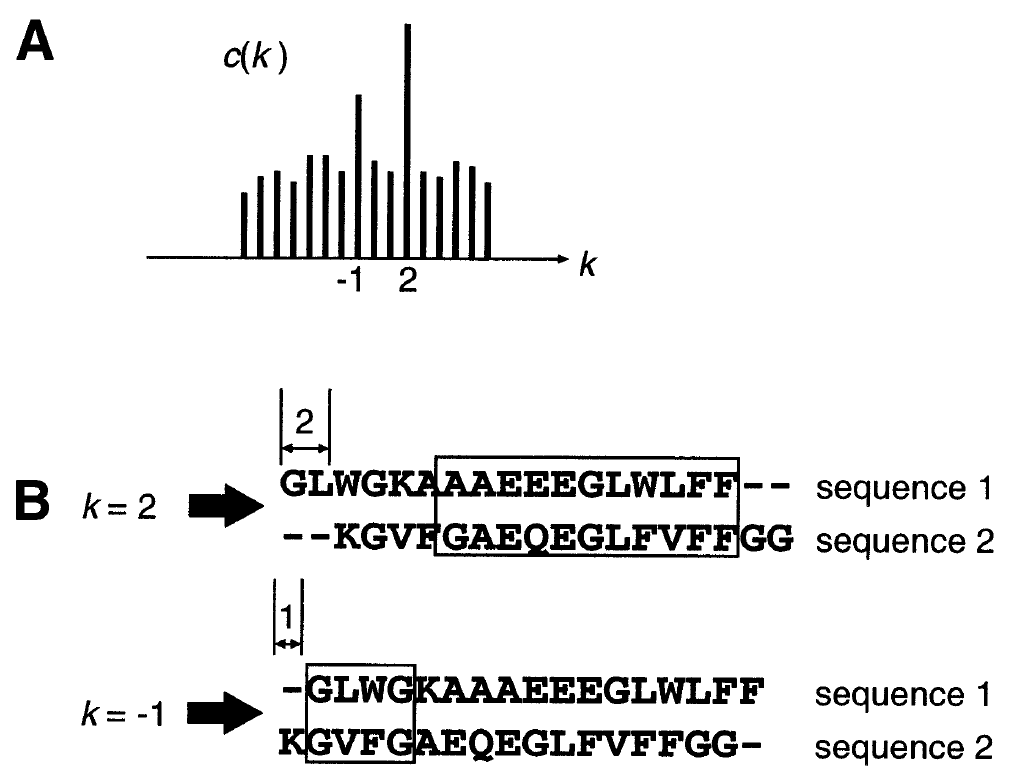
\includegraphics[width=0.5\textwidth]{./pictures/peaks.png}
  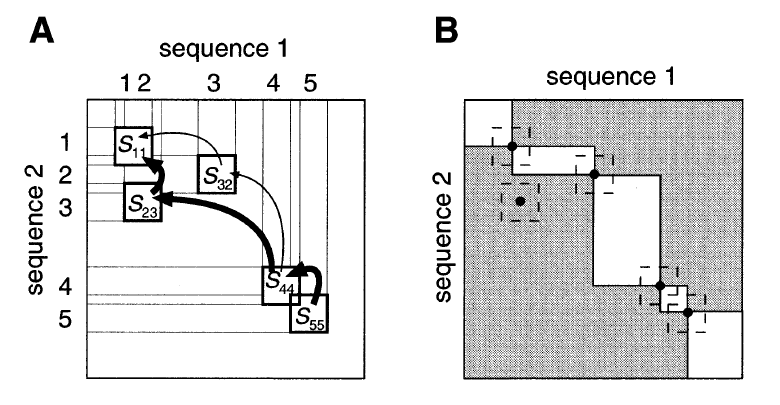
\includegraphics[width=0.5\textwidth]{./pictures/FFT.png}
  
  \begin{itemize}
  \item CPU time from $n^2$ to n $\cdot$ log n
  \item faster than T-coffee and ClustalW, same accuracy
  \end{itemize}
	\tiny{Nucleic Acids Res. 2002 Jul 15; 30(14): 3059–3066.}
}

%MAFFT is a multiple sequence alignment tool capable of performing aminoacid as well as nucleotid alignments, and is faster than similar algorithms like T-coffee or ClustalW by using the Fast Fourier Transform. Benchmark test showed that MAFFT results have the same accuracy than other tools, if similar homolog sequences are used, and reduces the CPU time from N square to N Log n.

\frame{
  \frametitle{RNAalifold}
  \begin{itemize}
  \item prediction of consensus structure for given alignment
  \item computation of MFE structures via RNAfold (recursive algorithm)
  \item thermodynamic energy minimization + simple scoring model (conservation score, gap elimination, structure constraints)
  \end{itemize}

}
	
\frame{
  \frametitle{RNAalifold}
  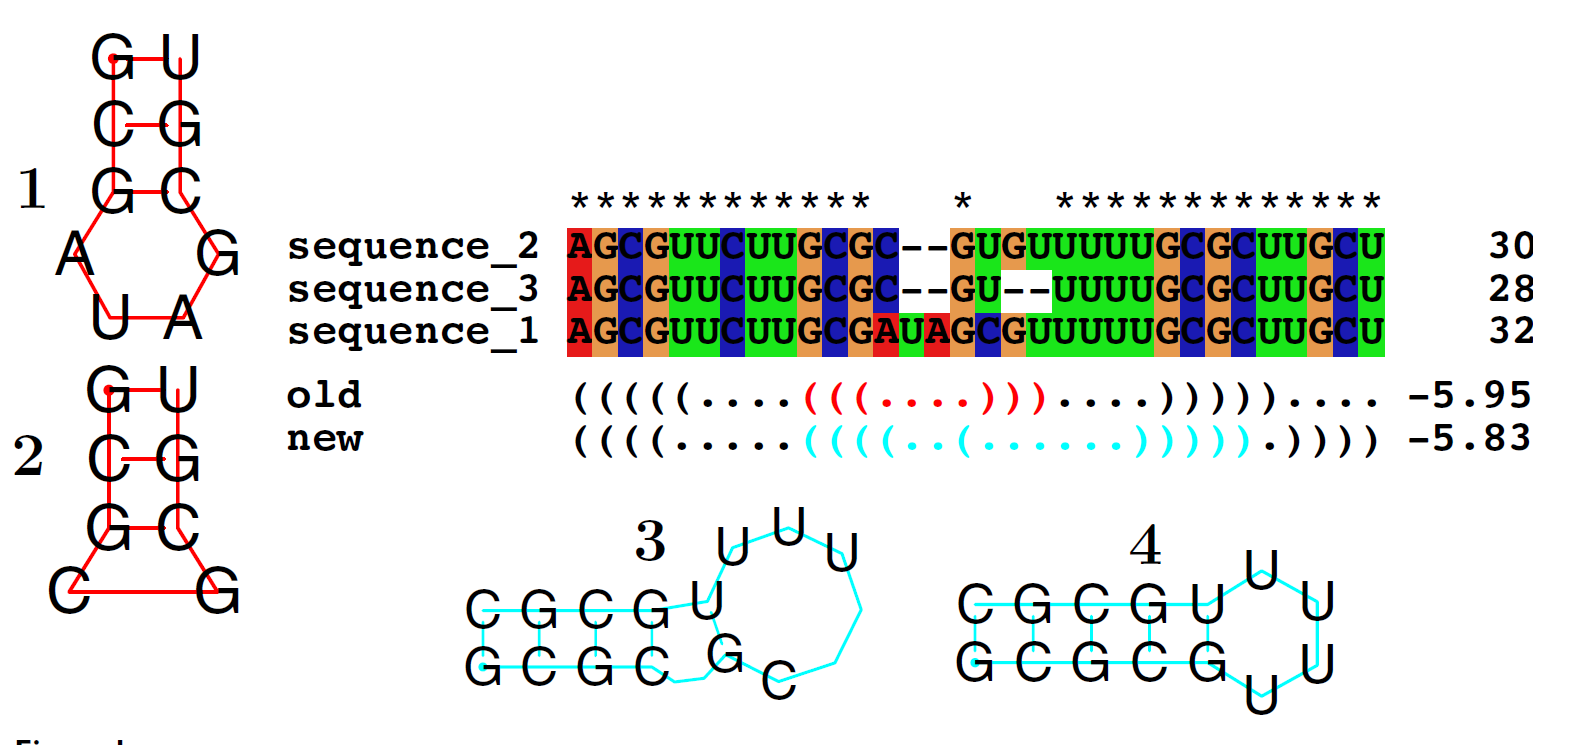
\includegraphics[width=0.9\textwidth]{./pictures/RNAalifold.png}
  \tiny{ doi:10.1186/1471-2105-9-474}

}


 
\frame{
\frametitle{Predictions}
	\begin{itemize}
	\item exons should be evolutionary conserved and could also have compensatory mutations
	\item exonic secondary structures should be unstable 
	\item introns experience less selective pressure, prone to accumulation of mutations
	\item intronic secondary structures should be stable, interaction with ribosome 
	\end{itemize}
}

%Exons are sequences that usually code for proteins within an organism, therefore they are put under a high selective pressure (conserved regions). In contrast introns are the sequences from the pre-mRNA, located between to exons, which are spliced out before the mature mRNA is exported into the cytoplasm. Introns therefore normally do not have any protein coding functionality. PHO1-2 antisense transcript introns are thought to be responsible for interactions with the ribosome, and should therefore be able to form more stable RNA secondary structures.
%- reversed complemantary intron regions are expected to be the most stable ones, as they do not bind to the mRNA, and might bind to the ribosome by forming stable secondary structures at the 3' end
%- forward strand as well as reversed complementary exon regions are not expected to form too stable secondary structure, as for one the ribosome will slide along the mRNA and in the case of the former ones, exonic regions in the antisense transcript could bind to the mRNA



\frame{
\frametitle{Results}
\begin{tabular}{l|l}
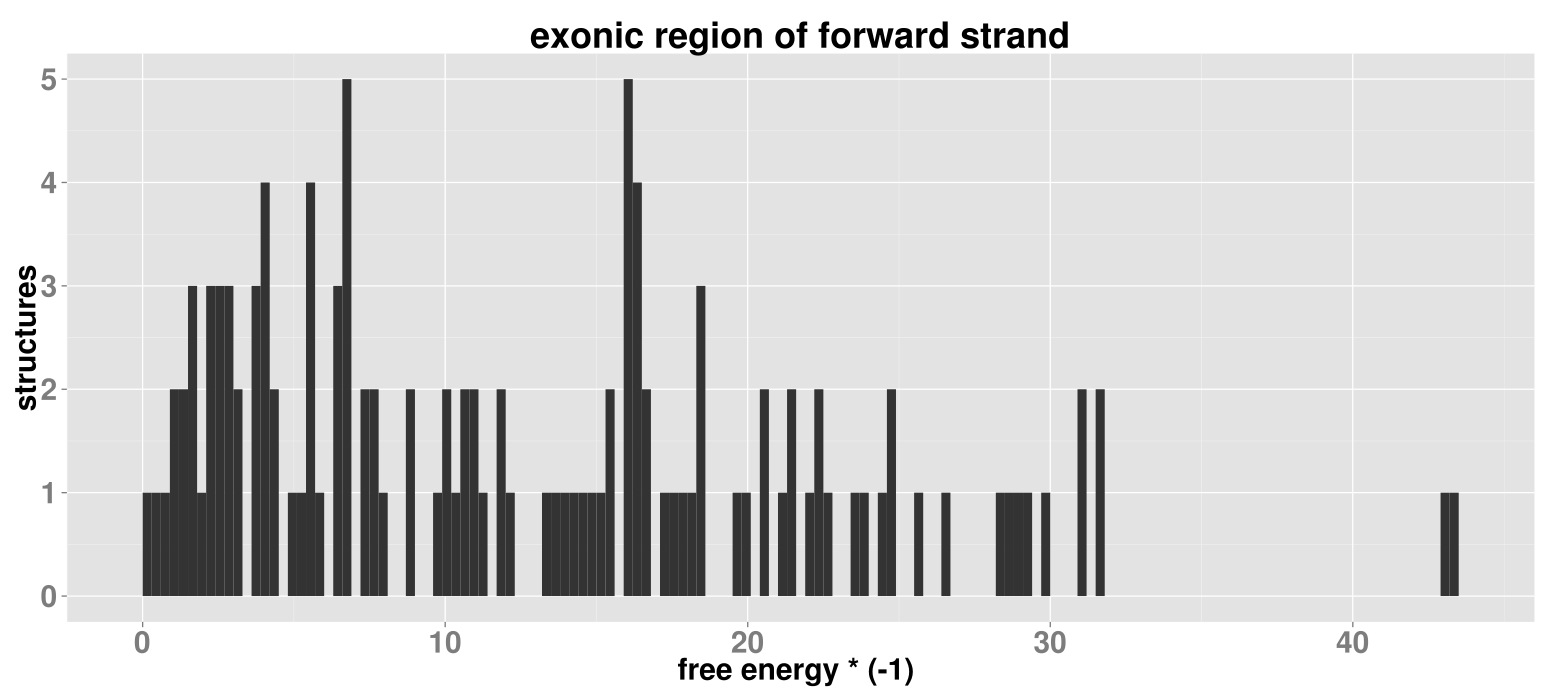
\includegraphics[width=0.5\textwidth]{./pictures/tableExonF.png} & 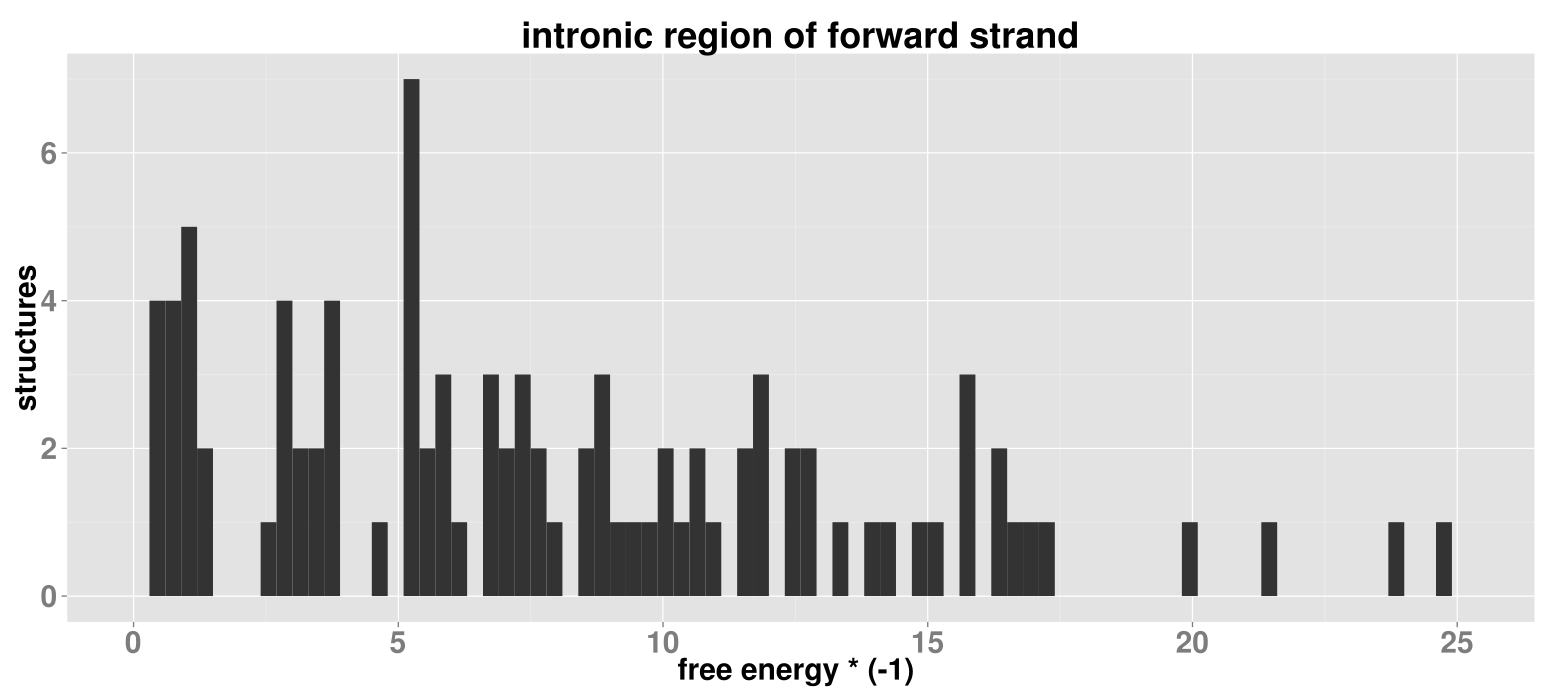
\includegraphics[width=0.5\textwidth]{./pictures/tableIntronF.png} \\ 
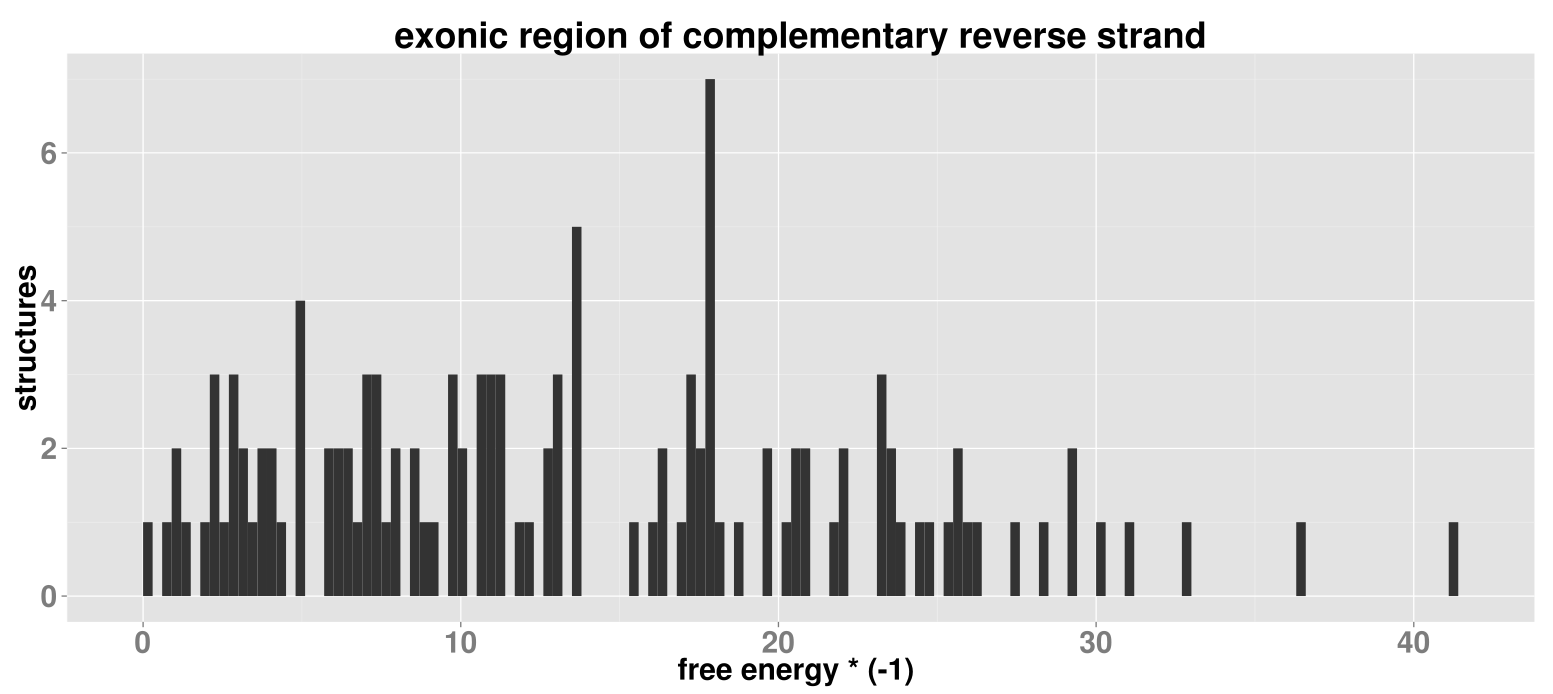
\includegraphics[width=0.5\textwidth]{./pictures/tableExonR.png} & 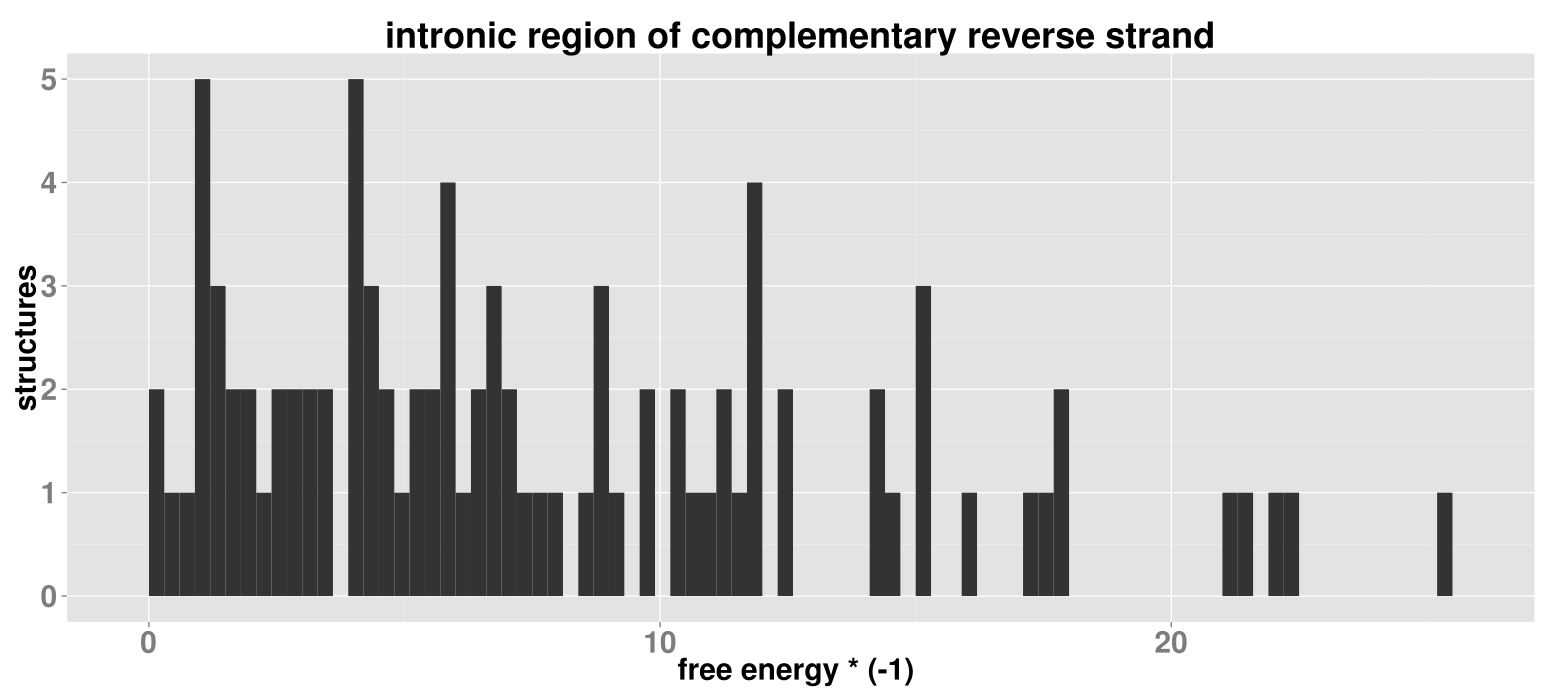
\includegraphics[width=0.5\textwidth]{./pictures/tableIntronR.png} \\
\end{tabular}
}


%Results
%Our analysis shows differences between the structural stability of RNA secondary structures between exons and introns in the forward strand as well as in the reversed strand. 
%It appears that exonic regions are more likely to form stable secondary structures than the intronic regions. There are some exonic structures which have a MFE greater than -30kcal/mol, whereas the intronic structure do not go under -25kcal/mol.
%
%Regarding exonic regions,the RNALalifold outputs shows that the most stable structure formed on the forward strand is located at alignment position of about 2000, and the most stable one for the reverse strand  located at position 4000. The alignment length is 6000 base-pairs, therefore the most stable structures on on the same position in the alignment. 


\frame{
\frametitle{Secondary structure visualization}
\begin{tabular}{l|l}

exonR MFE -40kcal/mol & exonR MFE -1kcal/mol \\
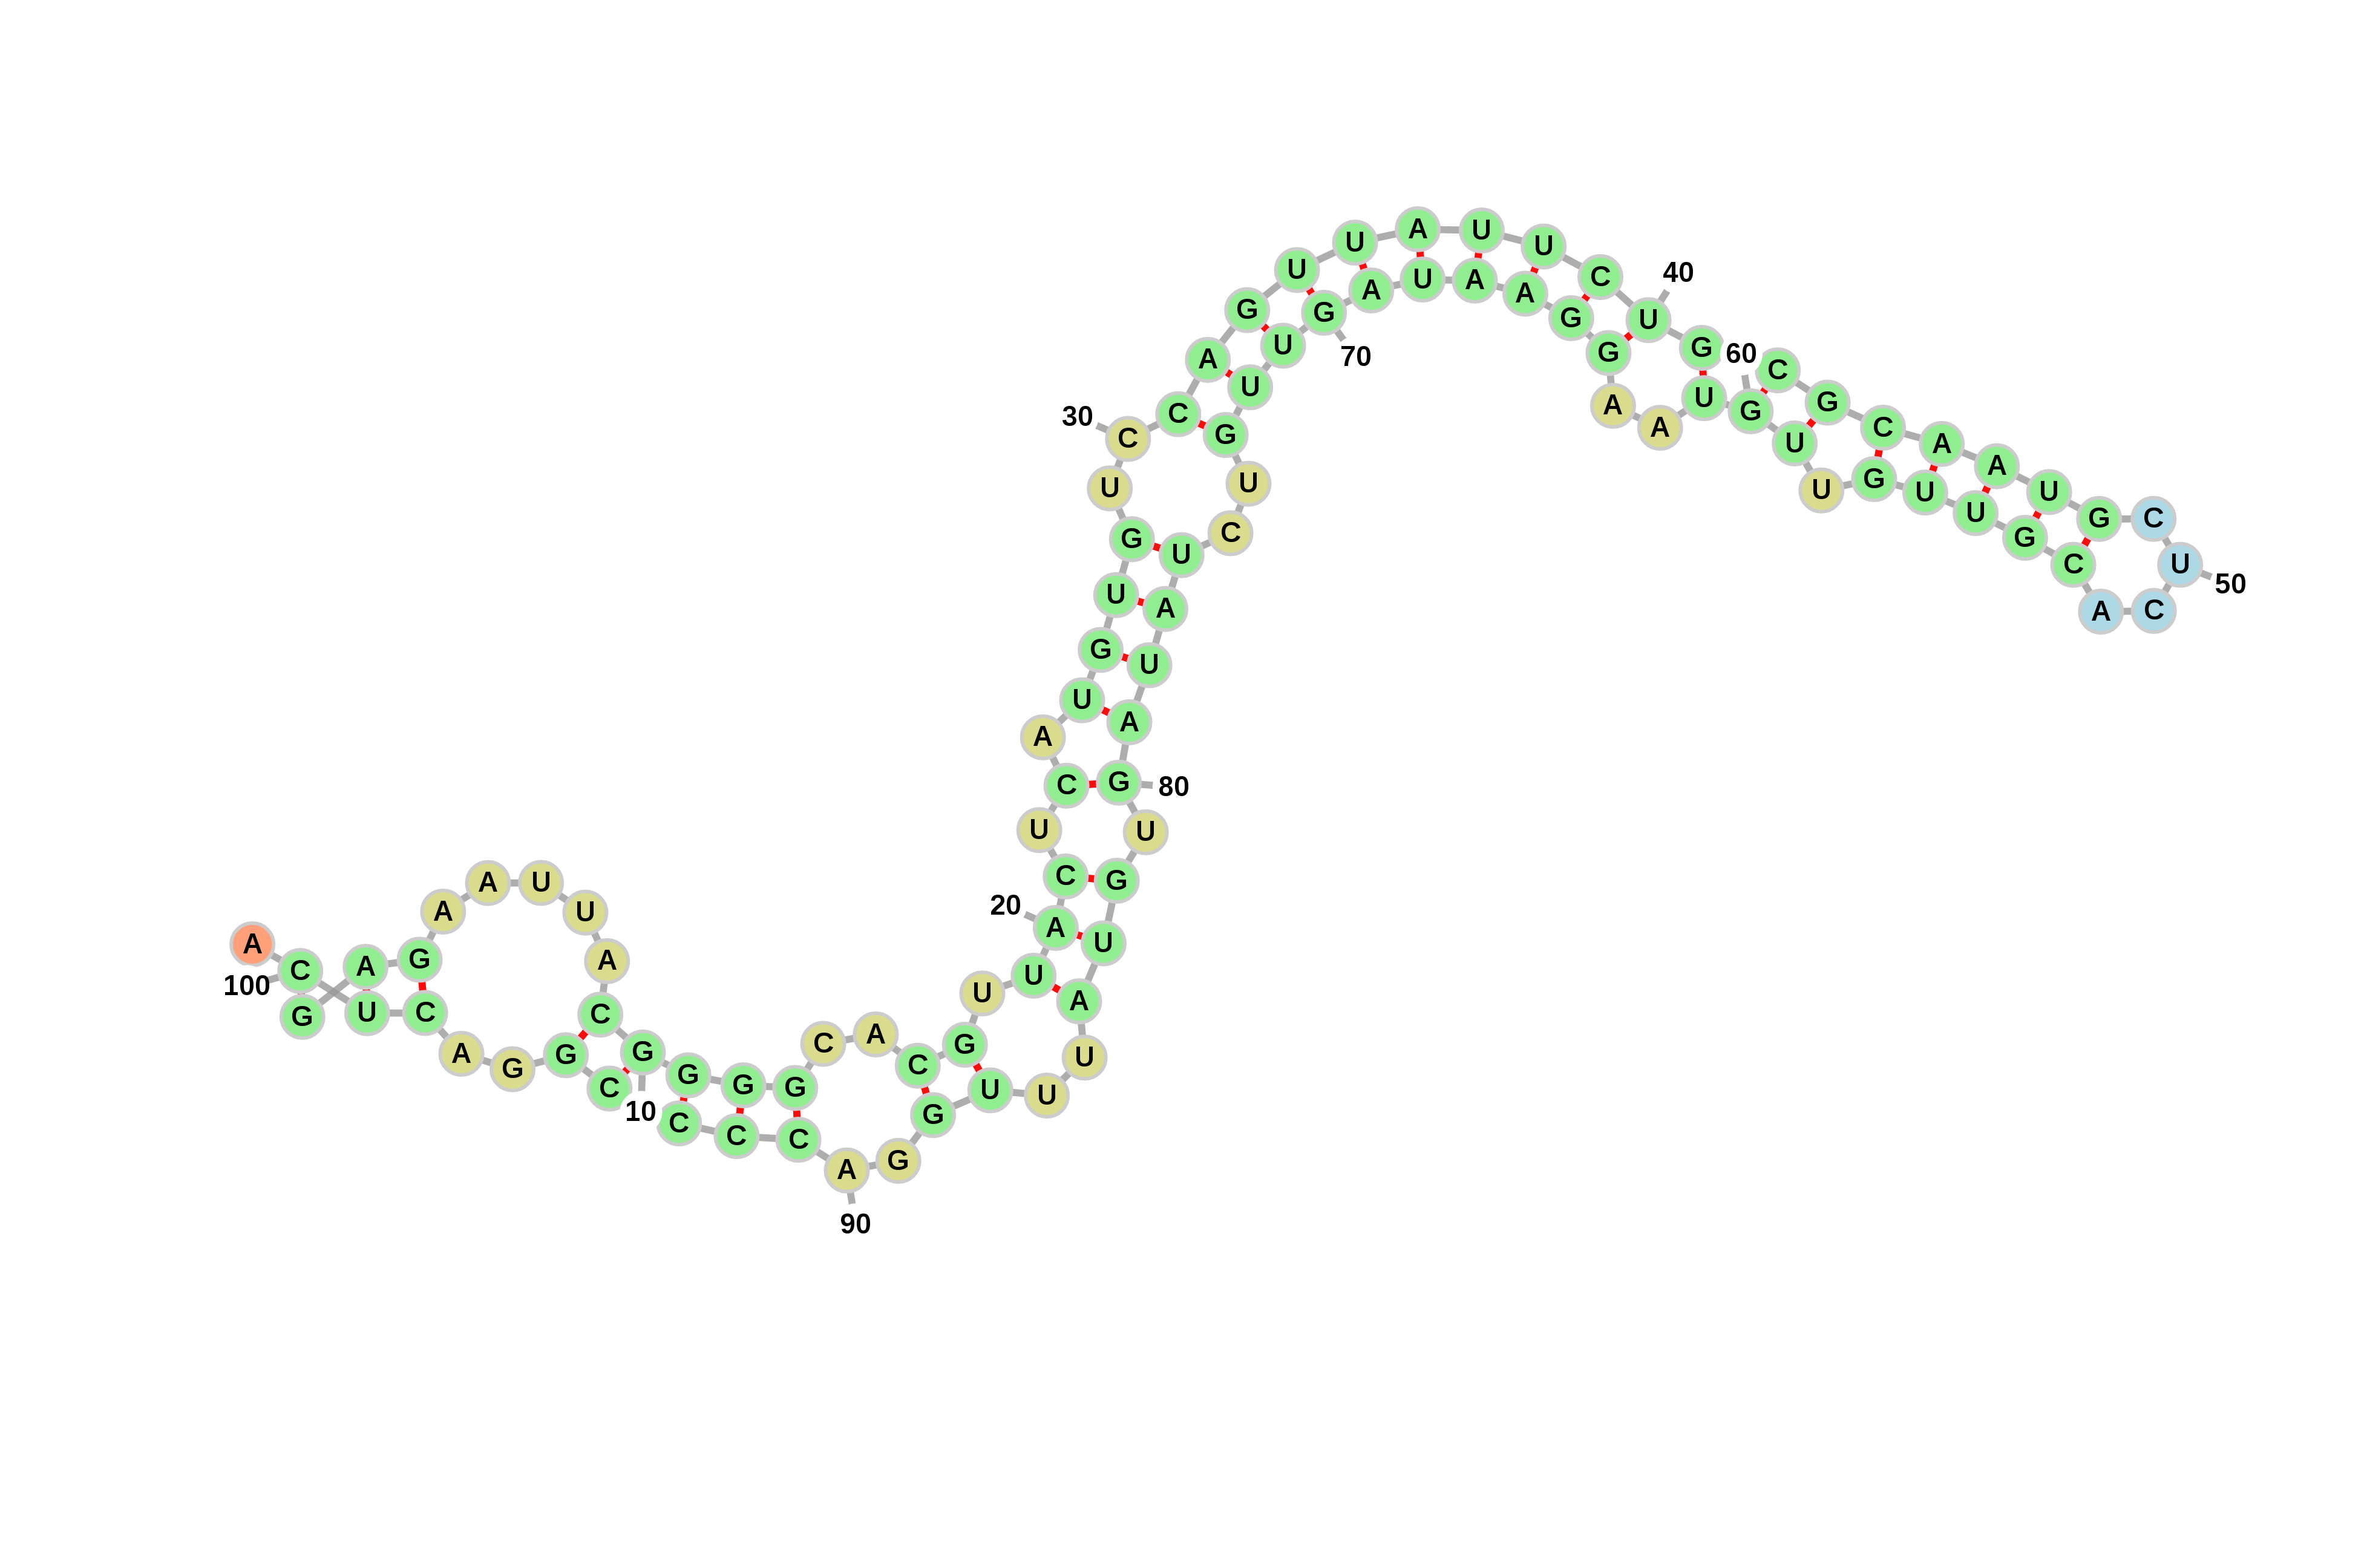
\includegraphics[width=0.5\textwidth]{./pictures/exonRstr1.png} &
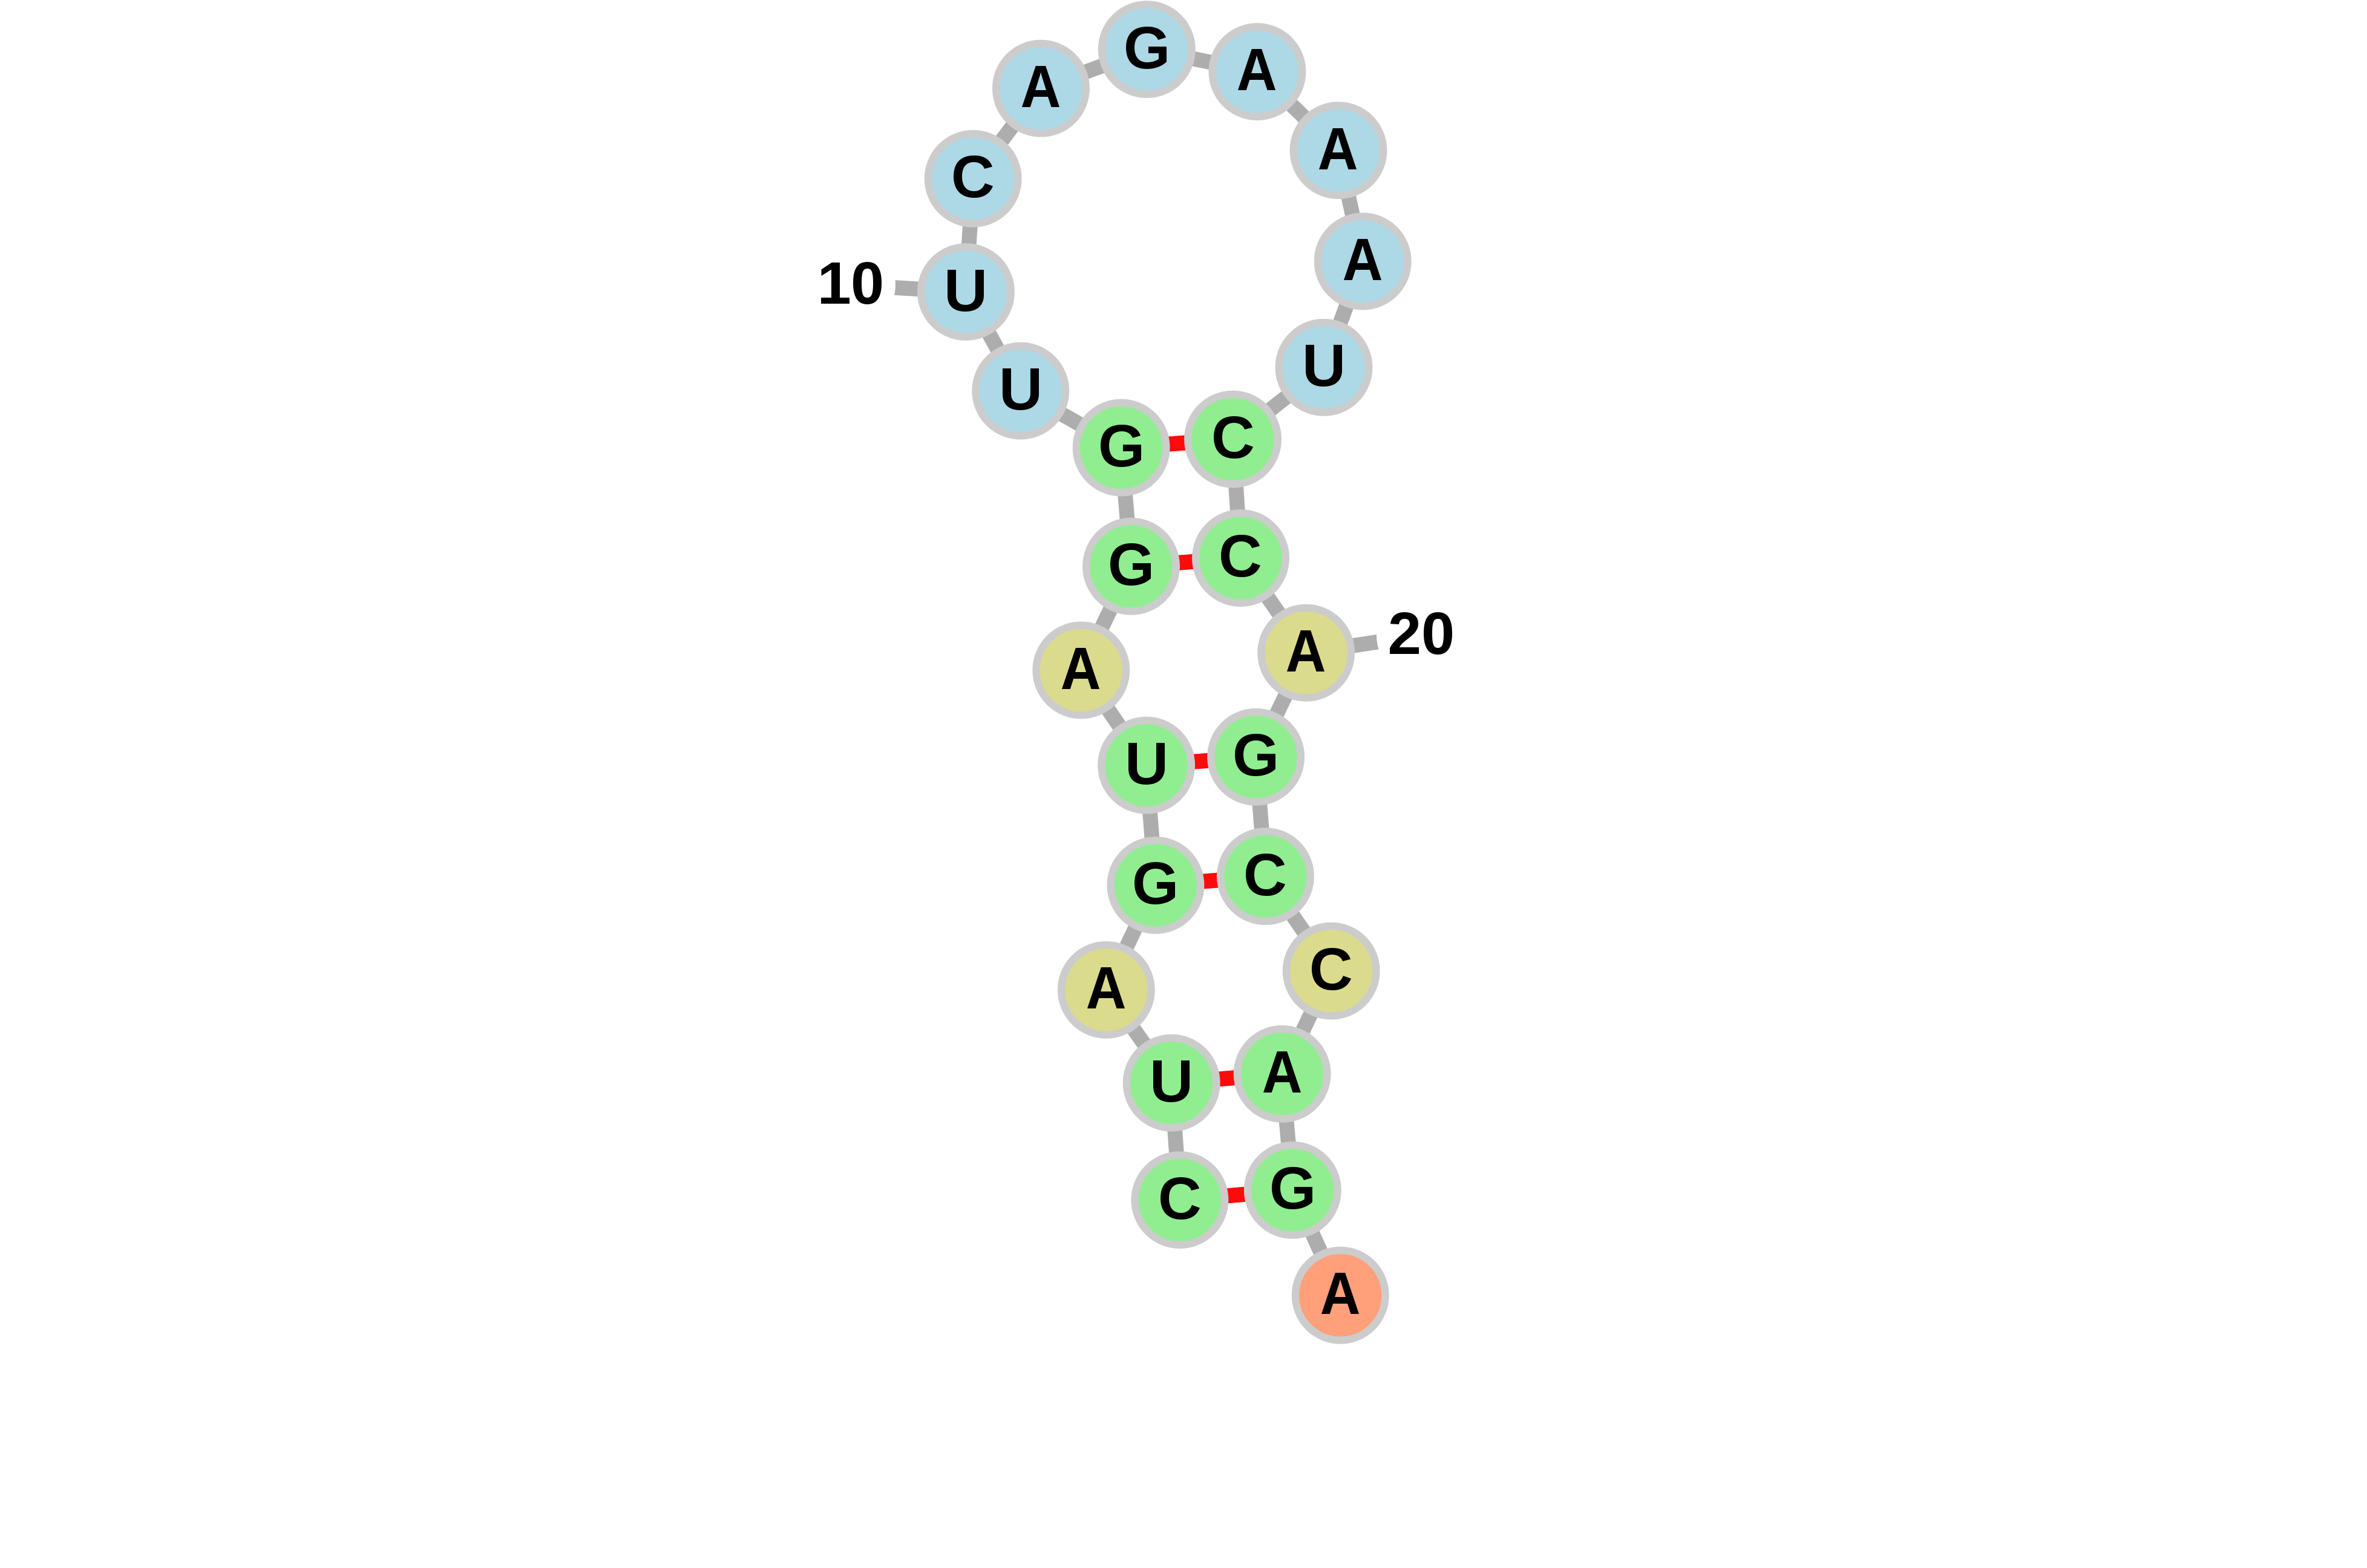
\includegraphics[width=0.5\textwidth]{./pictures/exonRstr2.png} \\
\end{tabular}
}

%It is just an overview of how secondary structures might look like if the MFE is eihter very high (unstable) or very low (stable). 



\frame{
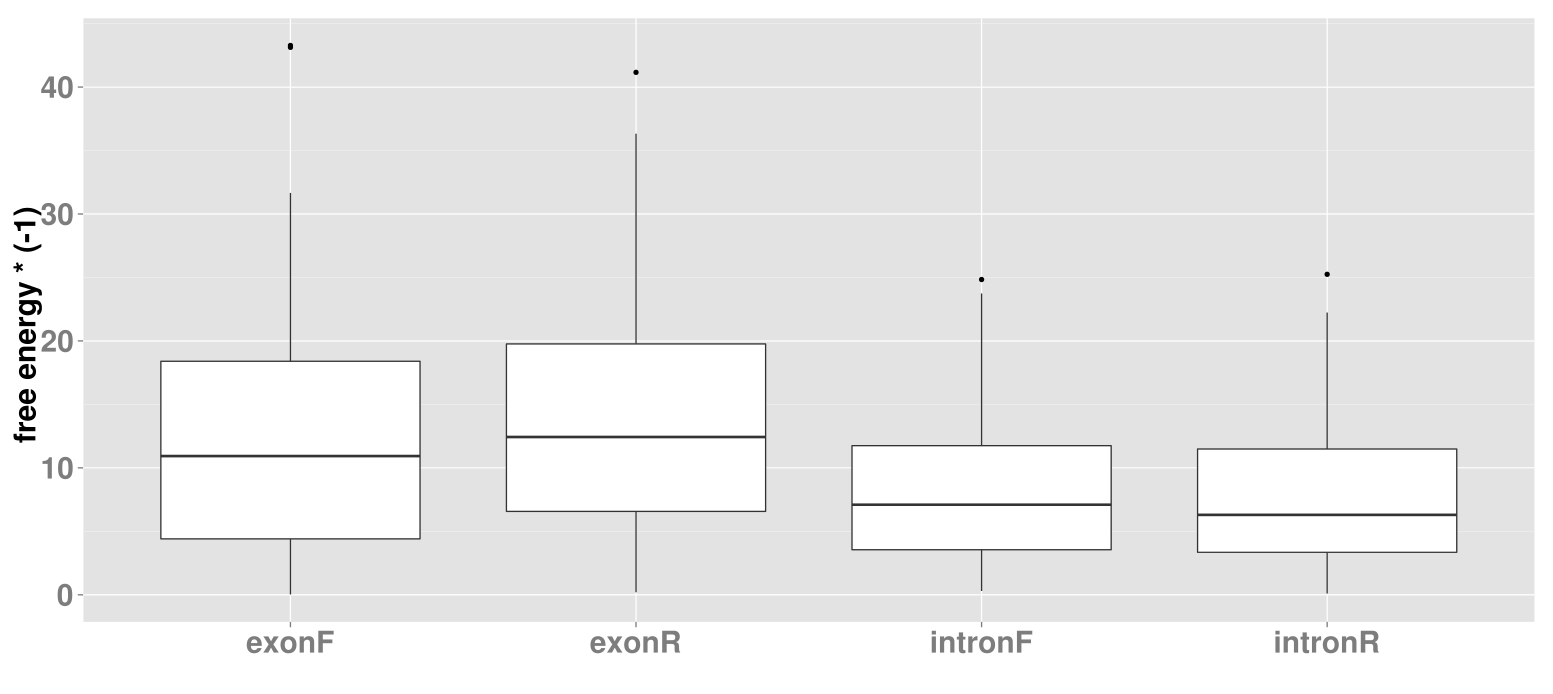
\includegraphics[width=1.0\textwidth]{./pictures/allTable.png} 
}

%same result as prior discussed. exonR forms slightly more stable structures than exonF.

\frame{
\frametitle{Discussion}
\begin{center}
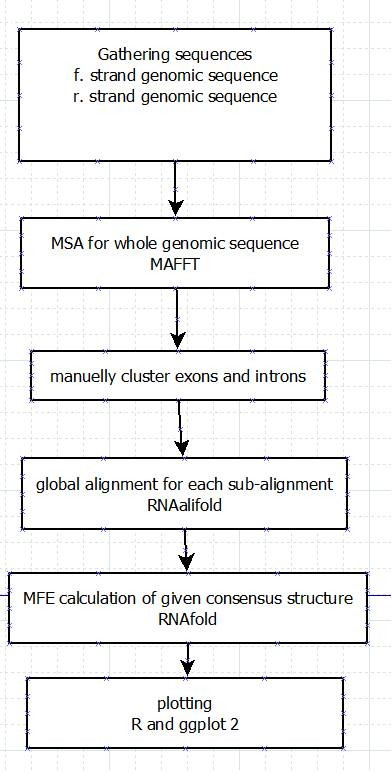
\includegraphics[width=0.3\textwidth]{./pictures/workFlow2.png} %!!!cahgne flowchart
\end{center}
}

%Due to the concatenation of exons and introns into one big sequence, and further using RNALalifold to detect local secondary structures will result with impossible structures prediction, and therefore distort the result. This impossible structures occur, when the  sequence of the found structure is part of 2 exons or 2 introns, meaning the sequence overlaps the concatenation gap.
% 
%For further studies, to eliminate this problem,  concatenation of exons and introns to one sequence should be avoided. This will change our flow-chart from prior to following. 
%A multiple sequence alignment is created for the whole genomic sequence + flanking regions. Afterwards single exonic as wellas intronic regions are picked out and and realigned with a global alignment program. The free energys of the resulting consensus structures can now be used for plotting




\end{document}
